%% LyX 2.2.2 created this file.  For more info, see http://www.lyx.org/.
%% Do not edit unless you really know what you are doing.
\documentclass[english]{article}
\usepackage[T1]{fontenc}
\usepackage[latin9]{inputenc}
\usepackage{geometry, graphicx}
\geometry{verbose,tmargin=3cm,bmargin=3cm,lmargin=3cm,rmargin=3cm}
\setlength{\parskip}{\bigskipamount}
\setlength{\parindent}{0pt}
\PassOptionsToPackage{normalem}{ulem}
\usepackage{ulem}
\usepackage{babel}
\pagenumbering{gobble}
\begin{document}
\textbf{Take Home Quiz 1 }

Official name (printed):\bigskip{}

Preferred name to be called: \bigskip{}

UIN: \bigskip{}

NetID: \bigskip{}

\textbf{\uline{Authorization to return graded papers}}:

Quizzes will be vertical-line folded with the grade inside the fold.
Exams will have the grade on an inside page. Both quizzes and exams
to be returned will be placed in piles at the front of the room alphabetized
by last name. Please indicate which one of the following is true:

\uline{\_\_\_\_\_\_\_} I agree to have my papers returned in this
manner.\bigskip{}

\uline{\_\_\_\_\_\_\_} I do not agree to have my papers returned
in this manner. Instead, I will pick up my papers in my instructor's
office during official office hours after they are returned to the
rest of the class.\bigskip{}

Signature: \uline{\_\_\_\_\_\_\_\_\_\_\_\_\_\_\_\_\_\_\_\_\_\_\_\_\_\_\_\_\_\_\_\_\_\_\_\_\_\_\_\_\_\_\_\_\_\_\_}\\

\vspace{1cm}

\newpage

1. A person will build a fence to enclose a rectangle of $2400$ square feet. The front of the fence is
made of a material priced at $\$20$ per linear foot. The other three sides are made of a material
priced at $\$12$ per foot of length. Find the cost of the fence as a function of the length of the
front.\\

Steps: Draw the rectangle and label the side lengths as x or y.
\vfill
Find the cost as a function of the two variables x and y.
\vfill


Use the fact that the area is 2400 to eliminate one of the variables.
\vfill

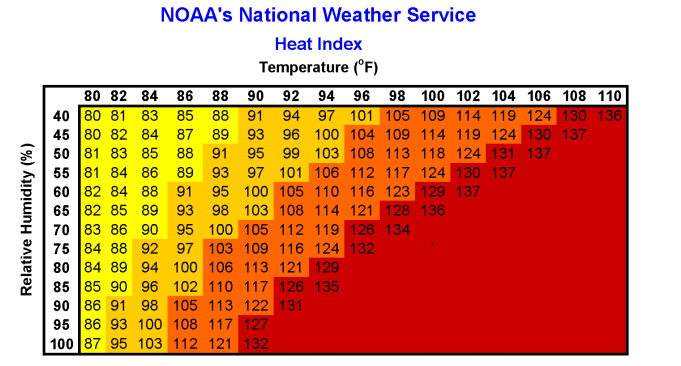
\includegraphics[width=0.8\textwidth,keepaspectratio]{nws}

2. (a) Find the linear regression for the heat index as a function of the relative humidity
at 80 degrees Fahrenheit (the leftmost column).

\vfill

(b) If the relative humidity increases by $10\%$ at 80 degrees Fahrenheit, how
much does the heat index increase by?

\vfill

\newpage

3. A drug is eliminated from the body at a rate proportional to the amount present.
A person took 16 mg at 7 pm on March 1. At 7pm on March 9 there were 4 mg remaining in the
body. 

a) Write the formula for the amount remaining $t$ days past 7 pm on March 1.
\vfill 

b) How much was left at 7 am on March 3? Round to 2 decimal places.
\vfill


4.  Find the domain of $\displaystyle f(x) = \sqrt{9 - x^2} + \frac {1}{1-x}$.

\vfill

5.  A person invests $\$10000$ into an account earning $4\%$ annual interest compounded continuously. 
The accumulated amount at the end of $t$ years is
$$A(t) = 10000 e^{0.04t}$$
In how many years, rounded to 3 decimal places, will the accumulated amount be $\$25000$?
\vfill
\end{document}
